\section*{Beispiel für eine Programmausführung}
\label{sec:program}
\lstset{language=C++,
	basicstyle=\ttfamily,
	keywordstyle=\color{blue}\ttfamily,
	stringstyle=\color{red}\ttfamily,
	commentstyle=\color{green}\ttfamily,
	morecomment=[l][\color{magenta}]{\#}
}
\begin{lstlisting}[frame=htrbl, caption={Implementierung von {\ttfamily main}}, label={lst:main}, basicstyle=\small]
#include <iostream>
#include <fstream>
#include "Manager.hpp"

int main()
{
  /*
   * Create variables and load UT as well as CT
   * It applies the following order: 4 < 3 < 2 < 1
   */
  Manager manager(4, 521, 521);
  BDDNode a( manager.createVariable(1) );
  BDDNode b( manager.createVariable(2) );
  BDDNode c( manager.createVariable(3) );
  BDDNode d( manager.createVariable(4) );
  // Create BDD by combinations (synthesis)
  BDDNode g = (a * b) ^ (!c + d);
  // Compute the high child of the first variable
  BDDNode f = g.getCofactor( 1, BDDNode::getHighFactor() );
  /**
   * Show information to the BDD
   * Compiling with DEBUG also displays 
   * information about references
   */
  std::cout << f;
  // Visualize the BDD
  std::ofstream file("f.dot");
  manager.printNode(f, "f", file);
  system("dot -o f.png -T png f.dot");
  // Perform a manual garbage collection
  manager.clear();
  return 0;
}
\end{lstlisting}
\begin{verbatim}
0x1006346e0 [4, ~, 2] ( 0x1006346c0 [3, -, 2] ( 0x100634ba0 [2, -, 4] 
( 0x1006348a0 [0, -, 16] 0x1006348a0 [0, +, 16, X] ) 0x100634ba0 
[2, +, 4, X] ) 0x100634ba0 [2, +, 4, X] ) 
#Knoten: 4
\end{verbatim}
\newpage
\begin{figure}[bth]
	\centering
	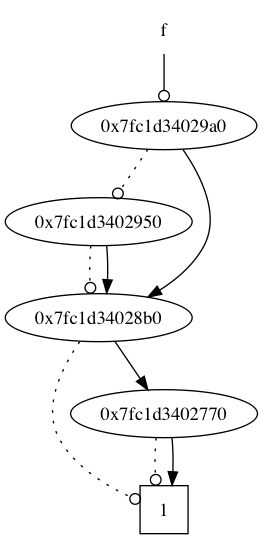
\includegraphics[scale=0.6]{./appendix/img/f}
	\caption[Visualisierung des BDDs nach der Programmausführung]{Visualisierung des BDDs nach der Programmausführung}
	\label{fig:vis}
\end{figure}
\noindent
\begin{verbatim}
digraph {
  node [shape=plaintext];
  terminal [label="1", shape=square];
  { rank=source; "f"; }
  node [shape=oval];
  "f" -> "0x7fc29b600d00" [arrowhead=odot]
  { rank=same; "0x7fc29b600d00"; }
  "0x7fc29b600d00" -> "0x7fc29b600ce0" [style=dotted];
  "0x7fc29b600d00" -> "0x7fc29b600c70";
  { rank=same; "0x7fc29b600ce0"; }
  "0x7fc29b600ce0" -> "0x7fc29b600c70" [style=dotted];
  "0x7fc29b600ce0" -> "0x7fc29b600c70";
  { rank=same; "0x7fc29b600c70"; }
  "0x7fc29b600c70" -> "terminal" [style=dotted];
  "0x7fc29b600c70" -> "terminal";
  { rank=same; "terminal"; }
}
\end{verbatim}
\section*{Auszug des Reports der Unittests}
\label{sec:unit}
\tiny
\begin{verbatim}
<Catch name="ibdd_test">
<Group name="ibdd_test">
<TestCase name="Scenario: Working method of the unique table" tags="[unique-table]" filename="agrabddTest.cpp" line="6">
<Section name="Given: Three nodes, one key and slots in the unique table" filename="agrabddTest.cpp" line="8">
<Section name="When: a node is added" filename="agrabddTest.cpp" line="21">
<Section name="Then: it should also be found" filename="agrabddTest.cpp" line="23">
<OverallResults successes="1" failures="0" expectedFailures="0"/>
</Section>
<OverallResults successes="1" failures="0" expectedFailures="0"/>
</Section>
<OverallResults successes="5" failures="0" expectedFailures="0"/>
</Section>
<Section name="Given: Three nodes, one key and slots in the unique table" filename="agrabddTest.cpp" line="8">
<Section name="When: a garbage collection is performed" filename="agrabddTest.cpp" line="27">
<Section name="Then: the unique table should be empty" filename="agrabddTest.cpp" line="29">
<OverallResults successes="1" failures="0" expectedFailures="0"/>
</Section>
<OverallResults successes="1" failures="0" expectedFailures="0"/>
</Section>
<OverallResults successes="5" failures="0" expectedFailures="0"/>
</Section>
<OverallResult success="true"/>
</TestCase>
<TestCase name="Scenario: Working method of the computed table" tags="[computed-table]" filename="agrabddTest.cpp" line="35">
<Section name="Given: Three nodes, one key and slots in the computed table" filename="agrabddTest.cpp" line="37">
<Section name="When: a node is added" filename="agrabddTest.cpp" line="50">
<Section name="Then: it should also be found" filename="agrabddTest.cpp" line="52">
<OverallResults successes="1" failures="0" expectedFailures="0"/>
</Section>
<OverallResults successes="1" failures="0" expectedFailures="0"/>
</Section>
<OverallResults successes="5" failures="0" expectedFailures="0"/>
</Section>
<Section name="Given: Three nodes, one key and slots in the computed table" filename="agrabddTest.cpp" line="37">
<Section name="When: a garbage collection is performed" filename="agrabddTest.cpp" line="56">
<Section name="Then: the computed table should be empty" filename="agrabddTest.cpp" line="58">
<OverallResults successes="1" failures="0" expectedFailures="0"/>
</Section>
<OverallResults successes="1" failures="0" expectedFailures="0"/>
</Section>
<OverallResults successes="5" failures="0" expectedFailures="0"/>
</Section>
<OverallResult success="true"/>
</TestCase>
<TestCase name="Scenario: Application of operations to BDDs" tags="[operator]" filename="agrabddTest.cpp" line="64">
<Section name="Given: Two BDDs und slots in the unique as well as computed table" filename="agrabddTest.cpp" line="66">
<Section name="When: the conjunction is applied" filename="agrabddTest.cpp" line="73">
<Section name="Then: three nodes should exist" filename="agrabddTest.cpp" line="75">
<OverallResults successes="1" failures="0" expectedFailures="0"/>
</Section>
<OverallResults successes="1" failures="0" expectedFailures="0"/>
</Section>
<OverallResults successes="3" failures="0" expectedFailures="0"/>
</Section>
<Section name="Given: Two BDDs und slots in the unique as well as computed table" filename="agrabddTest.cpp" line="66">
<Section name="When: the disjunction is applied" filename="agrabddTest.cpp" line="79">
<Section name="Then: three nodes should exist" filename="agrabddTest.cpp" line="81">
<OverallResults successes="1" failures="0" expectedFailures="0"/>
</Section>
<OverallResults successes="1" failures="0" expectedFailures="0"/>
</Section>
<OverallResults successes="3" failures="0" expectedFailures="0"/>
</Section>
<Section name="Given: Two BDDs und slots in the unique as well as computed table" filename="agrabddTest.cpp" line="66">
<Section name="When: the adjunction is applied" filename="agrabddTest.cpp" line="85">
<Section name="Then: three nodes should exist" filename="agrabddTest.cpp" line="87">
<OverallResults successes="1" failures="0" expectedFailures="0"/>
</Section>
<OverallResults successes="1" failures="0" expectedFailures="0"/>
</Section>
<OverallResults successes="3" failures="0" expectedFailures="0"/>
</Section>
<Section name="Given: Two BDDs und slots in the unique as well as computed table" filename="agrabddTest.cpp" line="66">
<Section name="When: the &quot;More than&quot; operator is applied" filename="agrabddTest.cpp" line="91">
<Section name="Then: three nodes should exist" filename="agrabddTest.cpp" line="93">
<OverallResults successes="1" failures="0" expectedFailures="0"/>
</Section>
<OverallResults successes="1" failures="0" expectedFailures="0"/>
</Section>
<OverallResults successes="3" failures="0" expectedFailures="0"/>
</Section>
<Section name="Given: Two BDDs und slots in the unique as well as computed table" filename="agrabddTest.cpp" line="66">
<Section name="When: the &quot;Less than&quot; operator is applied" filename="agrabddTest.cpp" line="97">
<Section name="Then: three nodes should exist" filename="agrabddTest.cpp" line="99">
<OverallResults successes="1" failures="0" expectedFailures="0"/>
</Section>
<OverallResults successes="1" failures="0" expectedFailures="0"/>
</Section>
<OverallResults successes="3" failures="0" expectedFailures="0"/>
</Section>
<Section name="Given: Two BDDs und slots in the unique as well as computed table" filename="agrabddTest.cpp" line="66">
<Section name="When: the XNOR operator is applied" filename="agrabddTest.cpp" line="103">
<Section name="Then: three nodes should exist" filename="agrabddTest.cpp" line="105">
<OverallResults successes="1" failures="0" expectedFailures="0"/>
</Section>
<OverallResults successes="1" failures="0" expectedFailures="0"/>
</Section>
<OverallResults successes="3" failures="0" expectedFailures="0"/>
</Section>
<Section name="Given: Two BDDs und slots in the unique as well as computed table" filename="agrabddTest.cpp" line="66">
<Section name="When: the NAND operator is applied" filename="agrabddTest.cpp" line="109">
<Section name="Then: three nodes should exist" filename="agrabddTest.cpp" line="111">
<OverallResults successes="1" failures="0" expectedFailures="0"/>
</Section>
<OverallResults successes="1" failures="0" expectedFailures="0"/>
</Section>
<OverallResults successes="3" failures="0" expectedFailures="0"/>
</Section>
<Section name="Given: Two BDDs und slots in the unique as well as computed table" filename="agrabddTest.cpp" line="66">
<Section name="When: the NOR operator is applied" filename="agrabddTest.cpp" line="115">
<Section name="Then: three nodes should exist" filename="agrabddTest.cpp" line="117">
<OverallResults successes="1" failures="0" expectedFailures="0"/>
</Section>
<OverallResults successes="1" failures="0" expectedFailures="0"/>
</Section>
<OverallResults successes="3" failures="0" expectedFailures="0"/>
</Section>
<Section name="Given: Two BDDs und slots in the unique as well as computed table" filename="agrabddTest.cpp" line="66">
<Section name="When: the NOT operator is applied" filename="agrabddTest.cpp" line="121">
<Section name="Then: two nodes should exist" filename="agrabddTest.cpp" line="123">
<OverallResults successes="1" failures="0" expectedFailures="0"/>
</Section>
<OverallResults successes="1" failures="0" expectedFailures="0"/>
</Section>
<OverallResults successes="3" failures="0" expectedFailures="0"/>
</Section>
<Section name="Given: Two BDDs und slots in the unique as well as computed table" filename="agrabddTest.cpp" line="66">
<Section name="When: the high child is computed" filename="agrabddTest.cpp" line="127">
<Section name="Then: one node should exist" filename="agrabddTest.cpp" line="129">
<OverallResults successes="1" failures="0" expectedFailures="0"/>
</Section>
<OverallResults successes="1" failures="0" expectedFailures="0"/>
</Section>
<OverallResults successes="3" failures="0" expectedFailures="0"/>
</Section>
<Section name="Given: Two BDDs und slots in the unique as well as computed table" filename="agrabddTest.cpp" line="66">
<Section name="When: the low child is computed" filename="agrabddTest.cpp" line="133">
<Section name="Then: one node should exist" filename="agrabddTest.cpp" line="135">
<OverallResults successes="1" failures="0" expectedFailures="0"/>
</Section>
<OverallResults successes="1" failures="0" expectedFailures="0"/>
</Section>
<OverallResults successes="3" failures="0" expectedFailures="0"/>
</Section>
<OverallResult success="true"/>
</TestCase>
<TestCase name="Scenario: BDDs with complement edges" tags="[complementEdges]" filename="agrabddTest.cpp" line="141">
<Section name="Given: Two BDDs und slots in the unique as well as computed table" filename="agrabddTest.cpp" line="143">
<Section name="When: the function f=!(a*b) exists" filename="agrabddTest.cpp" line="150">
<Section name="Then: the root node should have a complement edge" filename="agrabddTest.cpp" line="152">
<OverallResults successes="1" failures="0" expectedFailures="0"/>
</Section>
<OverallResults successes="1" failures="0" expectedFailures="0"/>
</Section>
<OverallResults successes="3" failures="0" expectedFailures="0"/>
</Section>
<Section name="Given: Two BDDs und slots in the unique as well as computed table" filename="agrabddTest.cpp" line="143">
<Section name="When: the function f=a*b exists" filename="agrabddTest.cpp" line="156">
<Section name="Then: the root node should not have a complement edge" filename="agrabddTest.cpp" line="158">
<OverallResults successes="1" failures="0" expectedFailures="0"/>
</Section>
<OverallResults successes="1" failures="0" expectedFailures="0"/>
</Section>
<OverallResults successes="3" failures="0" expectedFailures="0"/>
</Section>
<OverallResult success="true"/>
</TestCase>
<TestCase name="Scenario: Nodes and their references" tags="[referenceCounter]" filename="agrabddTest.cpp" line="164">
<Section name="Given: Four BDDs und slots in the unique as well as computed table" filename="agrabddTest.cpp" line="166">
<Section name="When: a node is created for a variable" filename="agrabddTest.cpp" line="177">
<Section name="Then: the cofactor should be a leaf" filename="agrabddTest.cpp" line="178">
<OverallResults successes="1" failures="0" expectedFailures="0"/>
</Section>
<OverallResults successes="1" failures="0" expectedFailures="0"/>
</Section>
<OverallResults successes="5" failures="0" expectedFailures="0"/>
</Section>
<Section name="Given: Four BDDs und slots in the unique as well as computed table" filename="agrabddTest.cpp" line="166">
<Section name="When: a combination of BDDs exists" filename="agrabddTest.cpp" line="182">
<Section name="Then: the root node should have been reused once" filename="agrabddTest.cpp" line="185">
<OverallResults successes="1" failures="0" expectedFailures="0"/>
</Section>
<OverallResults successes="1" failures="0" expectedFailures="0"/>
</Section>
<OverallResults successes="5" failures="0" expectedFailures="0"/>
</Section>
<OverallResult success="true"/>
</TestCase>
<OverallResults successes="69" failures="0" expectedFailures="0"/>
</Group>
<OverallResults successes="69" failures="0" expectedFailures="0"/>
</Catch>
\end{verbatim}
\normalsize
\newpage
\section*{ISCAS'85 Schaltkreise}
\label{sec:iscas85}
\subsection*{C432 27-Channel Interrupt Controller}
\label{sec:c432}
\begin{figure}[bth]
	\centering
	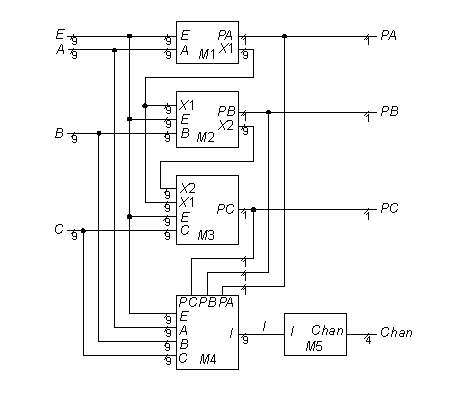
\includegraphics[scale=0.7]{./img/c432}
	\caption[C432 27-Channel Interrupt Controller]{C432 27-Channel Interrupt Controller \cite{h1999}}
	\label{fig:c432}
\end{figure}
\begin{table}[bth]
	\centering
	\caption{C432 27-Channel Interrupt Controller}
	\label{tab:c432}
	\begin{tabular}{ | p{2cm} | p{12cm} |}
		\hline
		\textbf{Statistik} & Es gibt 36 Eingänge, 7 Ausgänge und 160 Gatter. \\\hline
		\textbf{Funktion} & Die Eingänge \emph{A}, \emph{B} und \emph{C} werden in Busse gruppiert, die 9 Bit umfassen, wobei jedes Bit darin über die Anfrage-Priorität für einen Interrupt entscheidet. So haben Anfragen über \emph{A} immer eine höhere Priorität als Anfragen über \emph{B} bzw. \emph{C}. Sollten bspw. zwei Anfragen über $A$ vorliegen, so entscheidet der jeweilige Index über die priorisierte Behandlung. Ein höherer Index hat hierbei eine höhere Priorität. Der Bus \emph{E} wiederum aktiviert (und deaktiviert) die Interrupts hinsichtlich der jeweiligen Bitpositionen. Die Ausgänge \emph{PA}, \emph{PB}, \emph{PC} und \emph{Chan} spezifizieren dabei, welche Channels einen bestätigten Interrupt-Requests besitzen, wobei \emph{Chan} diese dekodiert.\\\hline
	\end{tabular}
\end{table}
\newpage
\subsection*{C499/C1355 32-Bit Single-Error-Correcting Circuit}
\label{sec:c499/c1355}
\begin{figure}[bth]
	\centering
	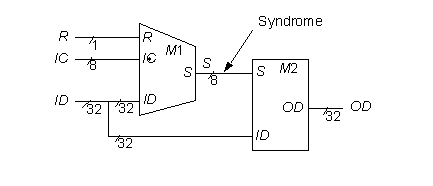
\includegraphics[scale=0.7]{./img/c499}
	\caption[C499/C1355 32-Bit Single-Error-Correcting Circuit]{C499/C1355 32-Bit Single-Error-Correcting Circuit \cite{h1999}}
	\label{fig:c499/c1355}
\end{figure}
\begin{table}[bth]
	\centering
	\caption{C499/C1355 32-Bit Single-Error-Correcting Circuit}
	\label{tab:c499/c1355}
	\begin{tabular}{ | p{2cm} | p{12cm} |}
		\hline
		\textbf{Statistik} & Es gibt 41 Eingänge, 32 Ausgänge und 202/546 Gatter. \\\hline
		\textbf{Funktion} & Der C499-Schaltkreis hat insgesamt gesehen die Aufgabe, Einzelfehler zu korrigieren. Die Eingänge werden hierzu kombiniert, um einen Bus \emph{S} zu erstellen, der 8 Bit besitzt. Anschließend erfolgt wiederum eine Kombination mit den 32 primären Eingängen, um die 32 primären Ausgänge zu bilden. Konkret betrachtet stellt \emph{S} eine Matrix für einen (40, 32)-Hamming-Code dar. Das Modul \emph{M1} erkennt hierbei einen Fehler, das Modul \emph{M2} hingegen kann diesen korrigieren. Der C1355-Schaltkreis hat dieselbe Funktionalität, jedoch sind hierbei alle XOR-Gatter durch die äquivalenten vier NAND-Gatter ersetzt worden.\\\hline
	\end{tabular}
\end{table}
\newpage
\subsection*{C880 8-Bit ALU}
\label{sec:c880}
\begin{figure}[bth]
	\centering
	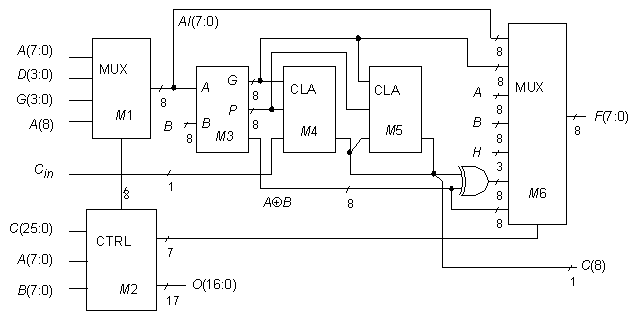
\includegraphics[scale=0.6]{./img/c880}
	\caption[C880 8-Bit ALU]{C880 8-Bit ALU \cite{h1999}}
	\label{fig:c880}
\end{figure}
\begin{table}[bth]
	\centering
	\caption{C880 8-Bit ALU}
	\label{tab:c880}
	\begin{tabular}{ | p{2cm} | p{12cm} |}
		\hline
		\textbf{Statistik} & Es gibt 60 Eingänge, 26 Ausgänge und 383 Gatter. \\\hline
		\textbf{Funktion} & Diese ALU stellt ein Rechenwerk dar, um Operationen zu berechnen. Welche konkrete Operation für Operanden eingesetzt wird, entscheiden die jeweiligen Multiplexer \emph{M1} und \emph{M6}, die wiederum von einem Mikrocode \emph{M2} kontrolliert werden.\\\hline
	\end{tabular}
\end{table}
\newpage
\subsection*{C1908 Single-Error-Correcting/Double-Error-Detecting Circuit}
\label{sec:c1908}
\begin{figure}[bth]
	\centering
	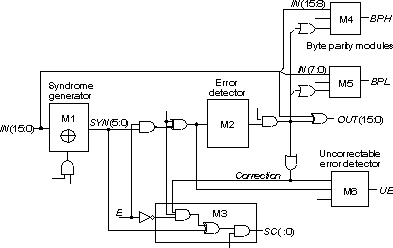
\includegraphics[scale=0.7]{./img/c1908}
	\caption[C1908 Single-Error-Correcting/Double-Error-Detecting Circuit]{C1908 Single-Error-Correcting/Double-Error-Detecting Circuit \cite{h1999}}
	\label{fig:c1908}
\end{figure}
\begin{table}[bth]
	\centering
	\caption{C1908 Single-Error-Correcting/Double-Error-Detecting Circuit}
	\label{tab:c1908}
	\begin{tabular}{ | p{2cm} | p{12cm} |}
		\hline
		\textbf{Statistik} & Es gibt 33 Eingänge, 25 Ausgänge und 880 Gatter. \\\hline
		\textbf{Funktion} & Dieser Schaltkreis kann Einzelfehler beheben und Doppelfehler erkennen. Er generiert 6-bit Syndrome aus einem 16-bit Eingang \emph{IN}, wobei dieser speziell dafür dekodiert wurde, um Bitfehler zu finden, insofern welche existieren. Wenn ein Fehler gefunden werden konnte und die Kontrolleingänge gesetzt sind, so wird dieser korrigiert. Zudem gibt es einen Ausgang, der anzeigt, ob es mehrere Fehler gibt, wobei diese dann nicht korrigiert werden können. \\\hline
	\end{tabular}
\end{table}
\newpage
\subsection*{C2670 12-bit ALU und Controller}
\label{sec:c2670}
\begin{figure}[bth]
	\centering
	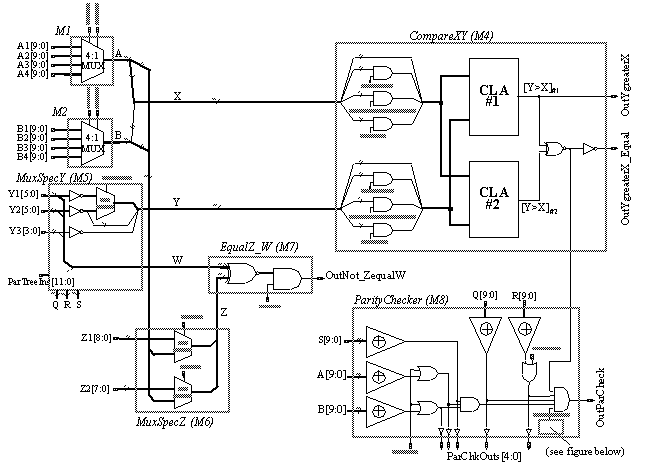
\includegraphics[scale=0.6]{./img/c2670}
	\caption[C2670 12-bit ALU und Controller]{C2670 12-bit ALU und Controller \cite{h1999}}
	\label{fig:c2670}
\end{figure}
\begin{table}[bth]
	\centering
	\caption{C2670 12-bit ALU und Controller}
	\label{tab:c2670}
	\begin{tabular}{ | p{2cm} | p{12cm} |}
		\hline
		\textbf{Statistik} & Es gibt 233 Eingänge, 140 Ausgänge und 1193 Gatter. \\\hline
		\textbf{Funktion} & Dieser Benchmark beinhaltet eine ALU mit einem Komparator, Äquivalenz-Checker und verschiedene Paritätsbäume. Der Komparator hat zwei 12-bit Eingänge \emph{X} sowie \emph{Y} und berechnet \emph{Y > X} durch die Benutzung von Carry-Lookahead Addierern. Gilt am Ausgang \emph{OutYgreaterX\_Equal} eine 1, so waren die Ausgänge der Addierer identisch, ansonsten ist das Ergebnis eine konstante 0. Das Modul \emph{M7} führt wiederum einen Äquivalenztest durch und das Modul \emph{M8} kennzeichnet den Paritätschecker, der Paritätsbäume enthält, die mithilfe einer Konjunktion kombiniert werden. \\\hline
	\end{tabular}
\end{table}
\newpage
\subsection*{C3540 8-bit ALU mit BCD-Arithmetik}
\label{sec:c3540}
\begin{figure}[bth]
	\centering
	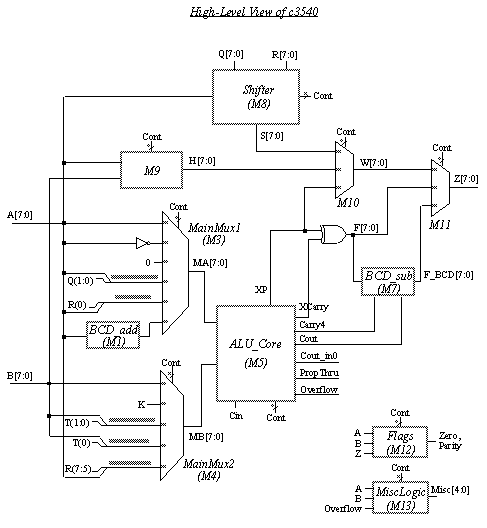
\includegraphics[scale=0.6]{./img/c3540}
	\caption[C3540 8-bit ALU mit BCD-Arithmetik]{C3540 8-bit ALU mit BCD-Arithmetik \cite{h1999}}
	\label{fig:c3540}
\end{figure}
\begin{table}[bth]
	\centering
	\caption{C3540 8-bit ALU mit BCD-Arithmetik}
	\label{tab:c3540}
	\begin{tabular}{ | p{2cm} | p{12cm} |}
		\hline
		\textbf{Statistik} & Es gibt 50 Eingänge, 22 Ausgänge und 1669 Gatter. \\\hline
		\textbf{Funktion} & Dieser Benchmark enthält eine 8-bit ALU, die arithmetische und logische Operationen auf binär kodierte Dezimalzahlen ausführen kann. Die Addition wird dabei z.\,B. durch einen Zweierkomplement-Addierer erledigt, der eine $6$ zu beiden Ziffern des ersten Operanden addiert und dann eine $6$ von den Ziffern des Ergebnisses subtrahiert, sollten diese keinen Carry produzieren. Das hierbei größte Modul ist \emph{M5}, das über zwei 4-bit Carry-Lookahead Addierern verfügt. \\\hline
	\end{tabular}
\end{table}
\newpage
\subsection*{C5315 9-bit ALU mit Paritätsberechnung}
\label{sec:c5315}
\begin{figure}[bth]
	\centering
	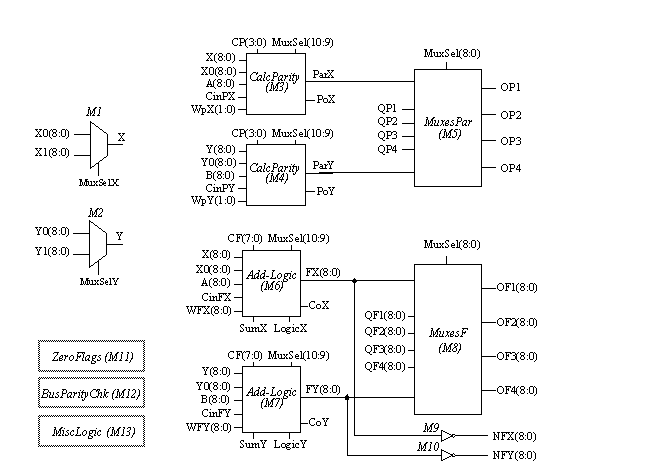
\includegraphics[scale=0.6]{./img/c5315}
	\caption[C5315 9-bit ALU mit Paritätsberechnung]{C5315 9-bit ALU mit Paritätsberechnung \cite{h1999}}
	\label{fig:c5315}
\end{figure}
\begin{table}[bth]
	\centering
	\caption{C5315 9-bit ALU mit Paritätsberechnung}
	\label{tab:c5315}
	\begin{tabular}{ | p{2cm} | p{12cm} |}
		\hline
		\textbf{Statistik} & Es gibt 178 Eingänge, 123 Ausgänge und 2403 Gatter. \\\hline
		\textbf{Funktion} & Bei diesem Schaltkreis handelt es sich um eine ALU, die simultan arithmetische und logische Operationen auf zwei 9-bit Eingängen ausführt und dazu die jeweilige Parität dieser Resultate berechnet. Die Module \emph{M6} und \emph{M7} berechnen hierbei die arithmetische oder logische Operation, die durch das Bauteil \emph{CF} spezifiziert wird. Das Modul \emph{M5} beinhaltet wiederum Multiplexer, die die jeweiligen Resultate weiterleitet. Die Module \emph{M3} und \emph{M4} sind hingegen dafür zuständig, die Parität des Resultates zu berechnen.\\\hline
	\end{tabular}
\end{table}
\newpage
\subsection*{C6288 16-bit Multiplizierer}
\label{sec:c6288}
\begin{figure}[bth]
	\centering
	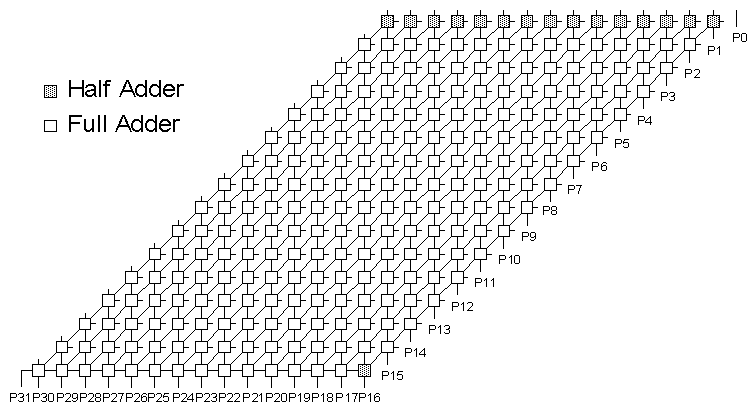
\includegraphics[scale=0.5]{./img/c6288}
	\caption[C6288 16-bit Multiplizierer]{C6288 16-bit Multiplizierer \cite{h1999}}
	\label{fig:c6288}
\end{figure}
\begin{table}[bth]
	\centering
	\caption{C6288 16-bit Multiplizierer}
	\label{tab:c6288}
	\begin{tabular}{ | p{2cm} | p{12cm} |}
		\hline
		\textbf{Statistik} & Es gibt 32 Eingänge, 32 Ausgänge und 2406 Gatter. \\\hline
		\textbf{Funktion} & Dieser Schaltkreis dient zur Multiplikation von zwei 16-bit Eingängen. Dabei kennzeichnen die 2406 Gatter 240 Voll- und Halbaddierer in Form von Zellen hinsichtlich einer 15x16 Matrix.\\\hline
	\end{tabular}
\end{table}
\newpage
\subsection*{C7552 32-bit Addierer/Komparator}
\label{sec:c7552}
\begin{figure}[bth]
	\centering
	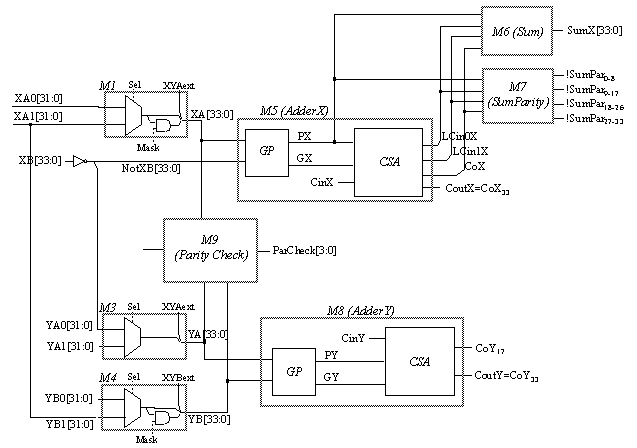
\includegraphics[scale=0.6]{./img/c7552}
	\caption[C7552 32-bit Addierer/Komparator]{C7552 32-bit Addierer/Komparator \cite{h1999}}
	\label{fig:c7552}
\end{figure}
\begin{table}[bth]
	\centering
	\caption{C7552 32-bit Addierer/Komparator}
	\label{tab:c7552}
	\begin{tabular}{ | p{2cm} | p{12cm} |}
		\hline
		\textbf{Statistik} & Es gibt 207 Eingänge, 108 Ausgänge und 3512 Gatter. \\\hline
		\textbf{Funktion} & Dieser Benchmark hat einen 34-bit Addierer (\emph{M5}), Komparator (\emph{M8}) und Paritätschecker (\emph{M9}). Jeder der Eingänge \emph{XA}, \emph{YA} und \emph{YB} wird von einer Menge von 2:1 Multiplexern bzw. deren SEL-Eingang versorgt. Der Komparator (\emph{M8}) verhält sich ähnlich zu dem Komparator von dem Schaltkreis \emph{C2670}, wobei die Addierer \emph{M5} und \emph{M8} sich identisch zu den Addierern des Schaltkreises \emph{C5315} verhalten.\\\hline
	\end{tabular}
\end{table}